
%(BEGIN_QUESTION)
% Copyright 2010, Tony R. Kuphaldt, released under the Creative Commons Attribution License (v 1.0)
% This means you may do almost anything with this work of mine, so long as you give me proper credit

A water-cooled generator at a power plant has two sources of cooling water flow, each source equipped with a flow switch that returns to its normally-open status if the water flow through the pipe stops.  If either water source ceases supplying cooling water to the generator (for whatever reason), that flow switch will de-actuate and turn the warning light on.  This is all that is required, as the generator will still receive adequate cooling from only one source.  If both water sources cease supplying water, however, a ``trip'' solenoid will de-energize to shut down the generator before it overheats:

$$\includegraphics[width=15.5cm]{i00046x01.eps}$$

One day the generator shuts down automatically, even though the warning light never came on.  An operator verifies that there is adequate cooling water flow going through both pipes.  Identify the likelihood of each specified fault for this circuit.  Consider each fault one at a time (i.e. no coincidental faults), determining whether or not each fault could independently account for {\it all} symptoms in this circuit.

% No blank lines allowed between lines of an \halign structure!
% I use comments (%) instead, so that TeX doesn't choke.

$$\vbox{\offinterlineskip
\halign{\strut
\vrule \quad\hfil # \ \hfil & 
\vrule \quad\hfil # \ \hfil & 
\vrule \quad\hfil # \ \hfil \vrule \cr
\noalign{\hrule}
%
% First row
{\bf Fault} & {\bf Possible} & {\bf Impossible} \cr
%
\noalign{\hrule}
%
% Another row
Solenoid coil failed open &  &  \cr
%
\noalign{\hrule}
%
% Another row
Flow switch A failed open &  &  \cr
%
\noalign{\hrule}
%
% Another row
Flow switch B failed open &  &  \cr
%
\noalign{\hrule}
%
% Another row
Open wire TP5-TP6 &  &  \cr
%
\noalign{\hrule}
%
% Another row
Open wire TP8-TP9 &  &  \cr
%
\noalign{\hrule}
%
% Another row
Open wire TP8-TP10 &  &  \cr
%
\noalign{\hrule}
%
% Another row
Relay coil CR1 failed open &  &  \cr
%
\noalign{\hrule}
%
% Another row
Relay coil CR2 failed open &  &  \cr
%
\noalign{\hrule}
} % End of \halign 
}$$ % End of \vbox

Finally, identify the {\it next} diagnostic test or measurement you would make on this system.  Explain how the result(s) of this next test or measurement help further identify the location and/or nature of the fault.

\vfil 

\underbar{file i00046}
\eject
%(END_QUESTION)





%(BEGIN_ANSWER)

This is a graded question -- no answers or hints given!

%(END_ANSWER)





%(BEGIN_NOTES)

We can tell by an analysis of the circuit that the shutdown solenoid is {\it de-energize to trip}.  Proper amounts of cooling water flow maintain both flow switches in their actuated (closed) states, maintaining power to the shutdown solenoid via the NO relay contacts.  Therefore, we may conclude that the solenoid shuts down the generator in the {\it absence} of applied power to it (i.e. if and when {\it both} flow switches go to their resting states, indicating no cooling water flow).

\vskip 10pt

Based on this analysis, we are looking for any sort of fault that could interrupt power from reaching the shutdown solenoid while not affecting the warning lamp.  This limits the domain of the fault to somewhere on the last rung of the circuit diagram:

% No blank lines allowed between lines of an \halign structure!
% I use comments (%) instead, so that TeX doesn't choke.

$$\vbox{\offinterlineskip
\halign{\strut
\vrule \quad\hfil # \ \hfil & 
\vrule \quad\hfil # \ \hfil & 
\vrule \quad\hfil # \ \hfil \vrule \cr
\noalign{\hrule}
%
% First row
{\bf Fault} & {\bf Possible} & {\bf Impossible} \cr
%
\noalign{\hrule}
%
% Another row
Solenoid coil failed open & $\surd$ &  \cr
%
\noalign{\hrule}
%
% Another row
Flow switch A failed open &  & $\surd$ \cr
%
\noalign{\hrule}
%
% Another row
Flow switch B failed open &  & $\surd$ \cr
%
\noalign{\hrule}
%
% Another row
Open wire TP5-TP6 &  & $\surd$ \cr
%
\noalign{\hrule}
%
% Another row
Open wire TP8-TP9 &  & $\surd$ \cr
%
\noalign{\hrule}
%
% Another row
Open wire TP8-TP10 & $\surd$ &  \cr
%
\noalign{\hrule}
%
% Another row
Relay coil CR1 failed open &  & $\surd$ \cr
%
\noalign{\hrule}
%
% Another row
Relay coil CR2 failed open &  & $\surd$ \cr
%
\noalign{\hrule}
} % End of \halign 
}$$ % End of \vbox

A good ``next test'' would be to measure AC voltage across the solenoid coil, to see if there is power applied.  If so, then the wiring is good and it is the solenoid that's failed.  If not, then the wiring is to blame for allowing the solenoid to become de-energized.


%INDEX% Switch, flow
%INDEX% Troubleshooting review: electric circuits

%(END_NOTES)


